\documentclass[Royal,times,sageh]{sagej}

\usepackage{moreverb,url,natbib, multirow, tabularx}
\usepackage[colorlinks,bookmarksopen,bookmarksnumbered,citecolor=red,urlcolor=red]{hyperref}



% tightlist command for lists without linebreak
\providecommand{\tightlist}{%
  \setlength{\itemsep}{0pt}\setlength{\parskip}{0pt}}



\usepackage{booktabs}
\usepackage{longtable}
\usepackage{array}
\usepackage{multirow}
\usepackage{wrapfig}
\usepackage{float}
\usepackage{colortbl}
\usepackage{pdflscape}
\usepackage{tabu}
\usepackage{threeparttable}
\usepackage{threeparttablex}
\usepackage[normalem]{ulem}
\usepackage{makecell}
\usepackage{xcolor}


\begin{document}


\setcitestyle{aysep={,}}

\title{TTS2016R: A data set to study population and employment patterns
from the 2016 Transportation Tomorrow Survey (TTS) in the Greater
Toronto and Hamilton Area in Canada}

\runninghead{}

\author{Anastasia Soukhov\affilnum{}, Antonio Paez\affilnum{}}

\affiliation{\affilnum{}{}}



\begin{abstract}
This paper describes and visualises the data contained within the
\{TTS2016R\} data-package created in \texttt{R}, the statistical
computing and graphics language. In addition to a synthetic example,
\{TTS2016R\} contains home-to-work commute information for the Greater
Golden Horseshoe area in Canada retrieved from the 2016 Transportation
Tomorrow Survey (TTS). Included are all Traffic Analysis Zones (TAZ),
the number of people who are employed full-time per TAZ, the number of
jobs per TAZ, and the origin and destination trips. \{TTS2016R\} also
includes the calculated car travel time from TAZ origin-destination
centroid pairs. This information is useful to understand patterns of
commuting in the region. We illustrate the estimation of a
distance-decay curve using these data. \{TTS2016R\} can be freely
downloaded and explored at: \url{https://github.com/soukhova/TTS2016R}
where the documentation and code involved in data creation,
manupulation, and the final data products are detailed.
\end{abstract}

\keywords{Jobs; population; travel time; impedance; Greater Toronto and
Hamilton Area; Ontario, Canada; R}

\maketitle

\hypertarget{introduction}{%
\section{Introduction}\label{introduction}}

This manuscript presents the open data product
\href{https://github.com/soukhova/TTS2016R}{\{TTS2016R\}}. Open data
products are the result of turning source data (open or otherwise) into
accessible information that adds value to the original inputs
\citep[see][]{Arribas2021open}. The product presented in this paper is
an \texttt{R} data package which currently consists of three objects
which are sourced from the 2016 Transportation Tomorrow Survey (TTS) or
are curated to facilitate the use and analysis of TTS data. This package
includes person-to-jobs origin-destinations, traffic analysis zone (TAZ)
boundaries, and planning/municipality boundaries for the Greater Golden
Horse area (GGH) located in southern Ontario, Canada
\citep{data_management_group_tts_2018}. In addition, the package
includes TAZ centroid-to-centroid travel times by car computed using
package \{r5r\} \citep{Pereira2021r5r}. The aim of this paper is to walk
readers through the empirical home-based work commute data set,
illustrate the calculation of an impedance function, showcase how it can
be used to calculate accessibility to employment, and invite its use in
other applications.

Data from the TTS are in principle available to the public but are not
fully open, since permission to access the data retrieval system is
required. In addition, the raw data can be technically demanding,
cumbersome to work with, and requires multiple software to process. By
pre-processing the data in a \texttt{R} environment, \{TTS2016R\} offers
a slice of the TTS data useful to understand patterns of commuting to
work in the region. It also provides open infrastructure for additional
TTS or complimentary data sets to be amended by the authors or wider
open-source community in the future.

\hypertarget{home-to-work-commute-data}{%
\section{Home-to-work commute data}\label{home-to-work-commute-data}}

\{TTS2016R\} includes counts of fully-employed population by place of
residence and counts of full-time jobs by place of work aggregated by
TAZ (n=3,764 within the survey boundaries). Unique identifiers use the
GTA06 Zoning System of TTS. The number of jobs (3,081,900) and workers
(3,446,957) are organized in the form of an origin-destination table,
indicative of patterns of home-to-work commute (there are 3,446,957
potential interactions). These data were retrieved from the
Transportation Tomorrow Survey Data Retrieval System on October 28, 2021
and reflect the potential interaction of full-time employed people and
jobs within the GGH survey boundaries shown in Figure
\ref{fig:TTS-16-survey-area} as defined by the 2016 TTS methodology
\citep{data_management_group_tts_2018}.

Also included in \{TTS2016R\} are travel times and cost of travel from
origin to destination by car; travel times are calculated using the
\texttt{R} package \{r5r\}. These travel times are useful to estimate
the cost of travel and to calculate impedance functions, among other
possible uses. It is important to note that for simplicity, all
interactions within \{TTS2016R\} are assumed to be taken by car, and the
travel time is calculated from an origin TAZ centroid to a destination
TAZ centroid. The centroid is snapped to the nearest street line by
\texttt{r5r} and the travel time is calculated for all trips assuming a
car travel mode. Additionally, only travel times less than or equal to
180 mins (3 hrs) are calculated; this threshold represents 99\% of
trip's travel times which are summarized in the descriptive statistics
in Table \ref{tab:TTS-16-desc-stats}.

\begin{figure}

{\centering 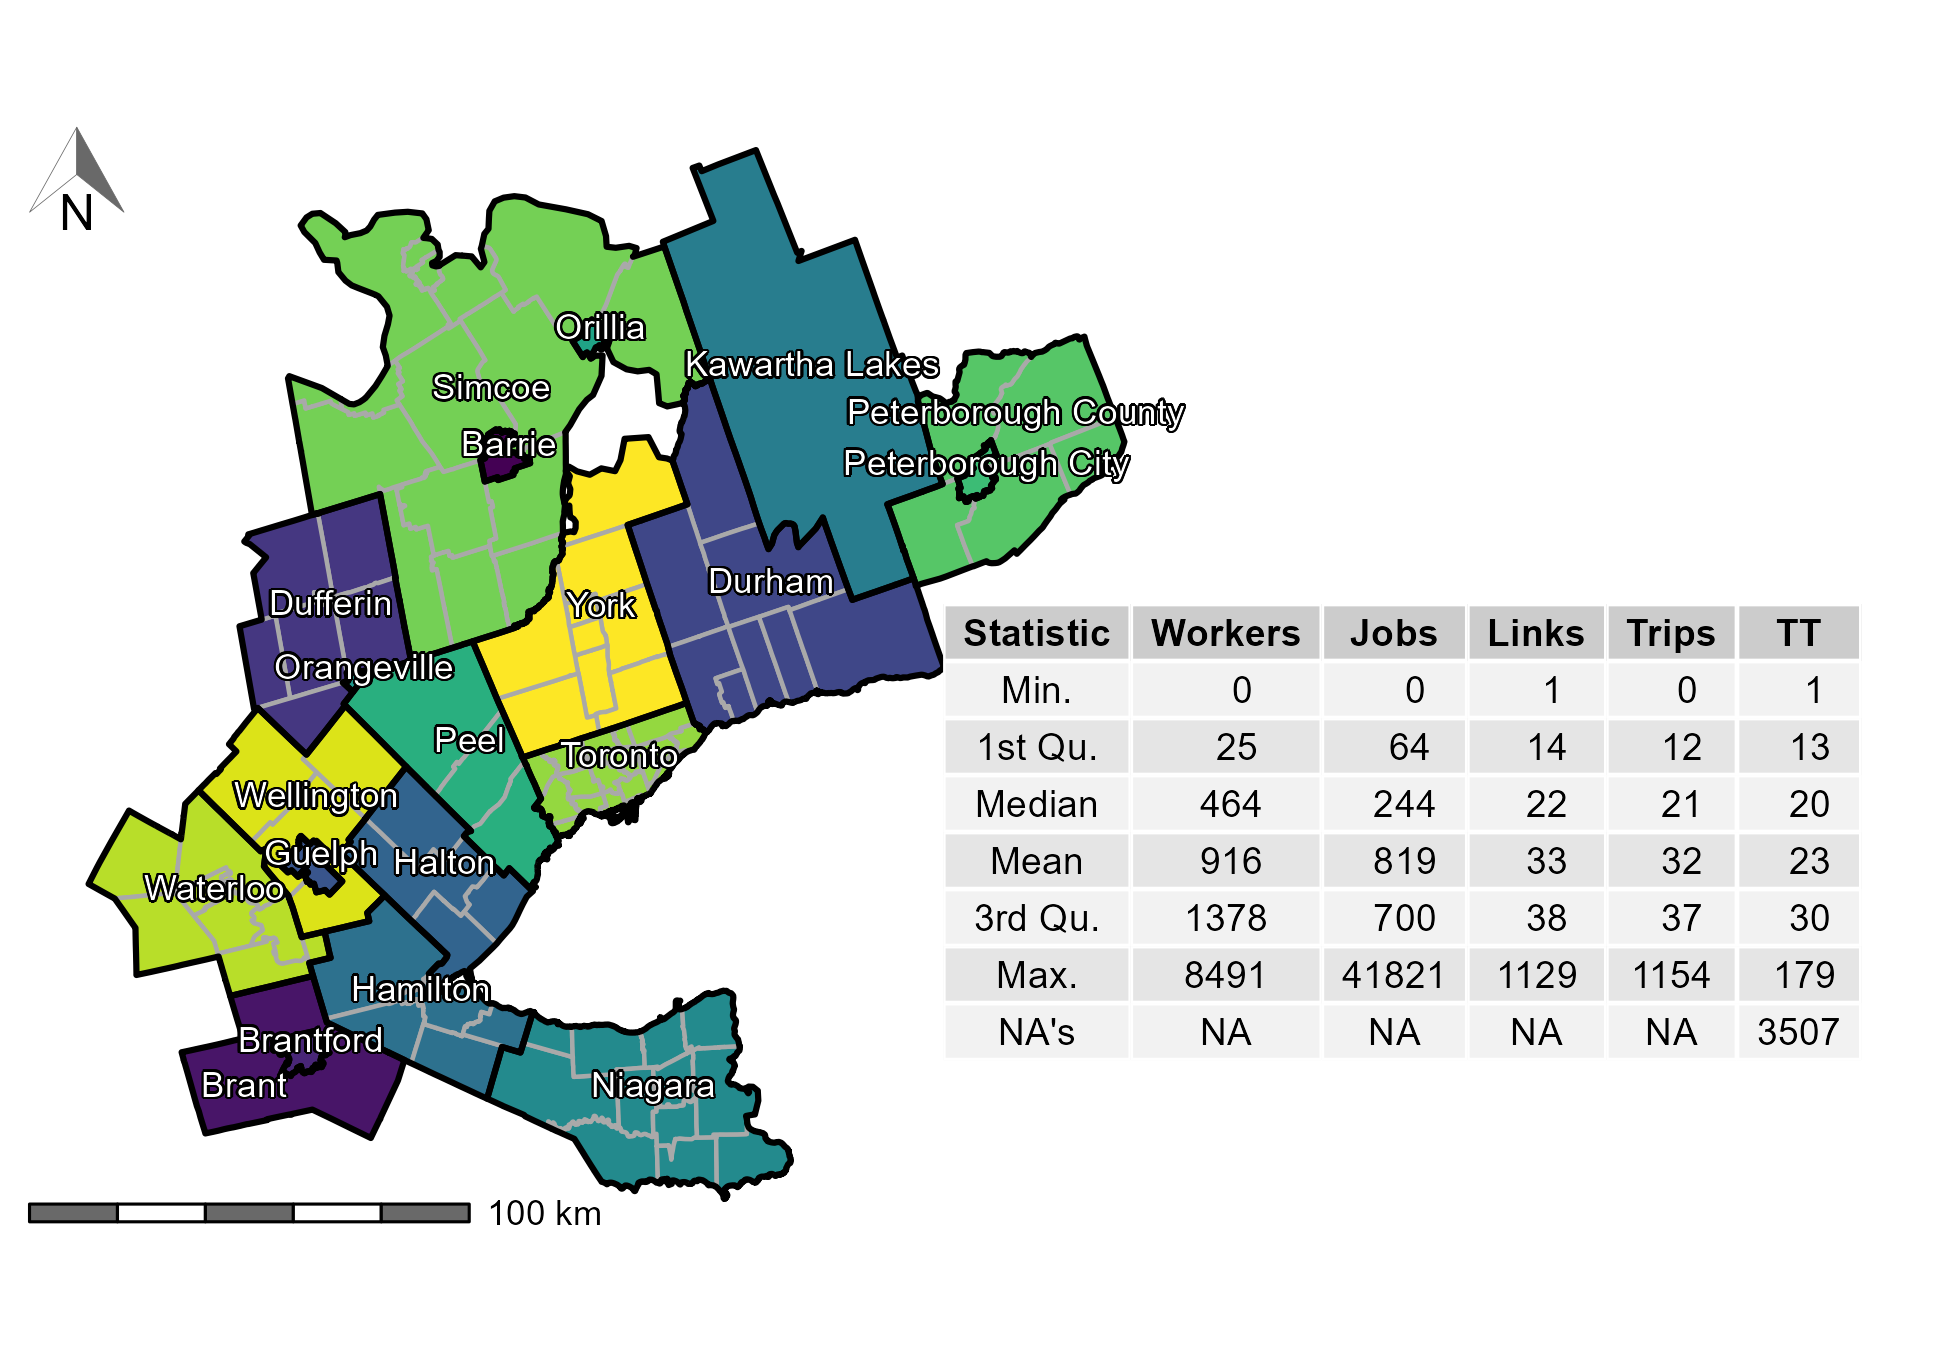
\includegraphics[width=0.8\linewidth]{images/TTS16-survey-area} 

}

\caption{\label{fig:TTS-16-survey-area}The TTS 2016 study area within the Greater Golden Horseshoe in Ontario, Canada.}\label{fig:TTS-16-survey-area}
\end{figure}

\begin{table}

\caption{\label{tab:creating-desc-stats-table}\label{tab:TTS-16-desc-stats}Descriptive statistics of the trips, workers, and jobs for the traffic analysis zones (TAZ) from the TTS 2016 dataset along with estimated car origin-destination travel times.}
\centering
\resizebox{\linewidth}{!}{
\begin{tabu} to \linewidth {>{\raggedright}X>{\raggedleft}X>{\raggedleft}X>{\raggedleft}X>{\raggedleft}X>{\raggedleft}X}
\toprule
\multicolumn{1}{r}{ } & \multicolumn{1}{r}{Trips} & \multicolumn{1}{r}{Car Travel Time} & \multicolumn{1}{r}{Area} & \multicolumn{1}{r}{Workers} & \multicolumn{1}{r}{Jobs} \\
\cmidrule(l{3pt}r{3pt}){2-2} \cmidrule(l{3pt}r{3pt}){3-3} \cmidrule(l{3pt}r{3pt}){4-4} \cmidrule(l{3pt}r{3pt}){5-5} \cmidrule(l{3pt}r{3pt}){6-6}
  & (\#) & (min) & (km\textasciicircum{}2) & (\#) & (\#)\\
\midrule
Min. & 1 & 0 & 0 & 0 & 0\\
1st Qu. & 14 & 13 & 1 & 25 & 64\\
Median & 22 & 20 & 1 & 464 & 244\\
Mean & 33 & 23 & 7 & 916 & 819\\
3rd Qu. & 38 & 30 & 3 & 1378 & 700\\
\addlinespace
Max. & 1129 & 179 & 879 & 8491 & 41821\\
NA's & NA & 3507 & NA & NA & NA\\
\bottomrule
\end{tabu}}
\end{table}

\hypertarget{employed-individuals-and-jobs}{%
\subsection{Employed individuals and
jobs}\label{employed-individuals-and-jobs}}

The origin-destination information consists of a cross-tabulation of
people who are employed full-time by place of residence (origin) and
places of employment in the GGH (destination) using the GTA06 zoning
system. The number of workers and jobs is not equal; the boundaries of
the survey are permeable, so workers who reside within the boundaries
but travel outside of the boundaries are counted as workers within an
origin TAZ, while jobs in TAZ that are filled by workers who reside
outside the GGH boundaries are \emph{unknown} since they were not
surveyed. This mismatch results in the total number of workers being
1.12 times larger than the number of jobs (i.e., 3,446,957 workers to
3,081,900 jobs). While the 2016 TTS survey boundaries are drawn to
minimize the difference between opportunities at the destination and
supply at the origins they are still not equal . That said, these data
offer a perspective of the potential of home-based trips to places of
employment and as such, the number of trips taken are equal to the
number of workers in the GGH.

\begin{figure}
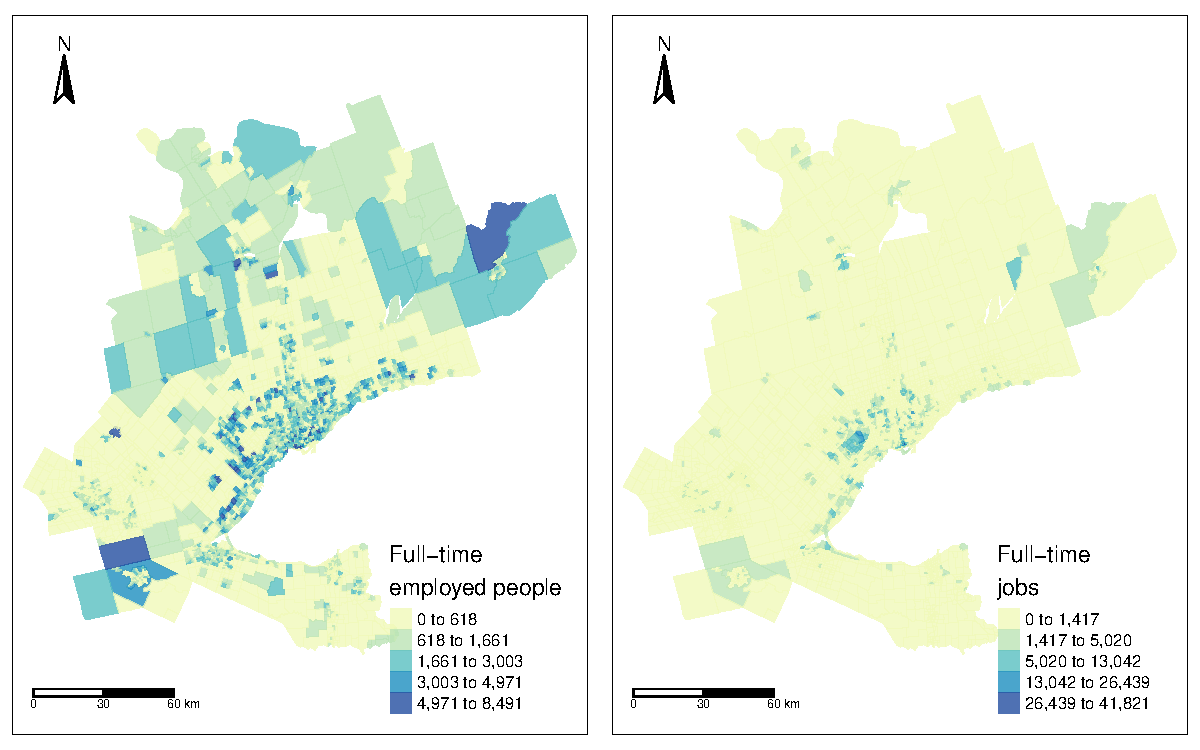
\includegraphics[width=1\linewidth]{Manuscript-Data-Package_files/figure-latex/tts-workers-jobs-plot-1} \caption{\label{fig:tts-workers-jobs-plot}Number of workers (top) and jobs (bottom) in each TAZ in the GGH area as specified in the 2016 TTS.}\label{fig:tts-workers-jobs-plot}
\end{figure}

\begin{figure}
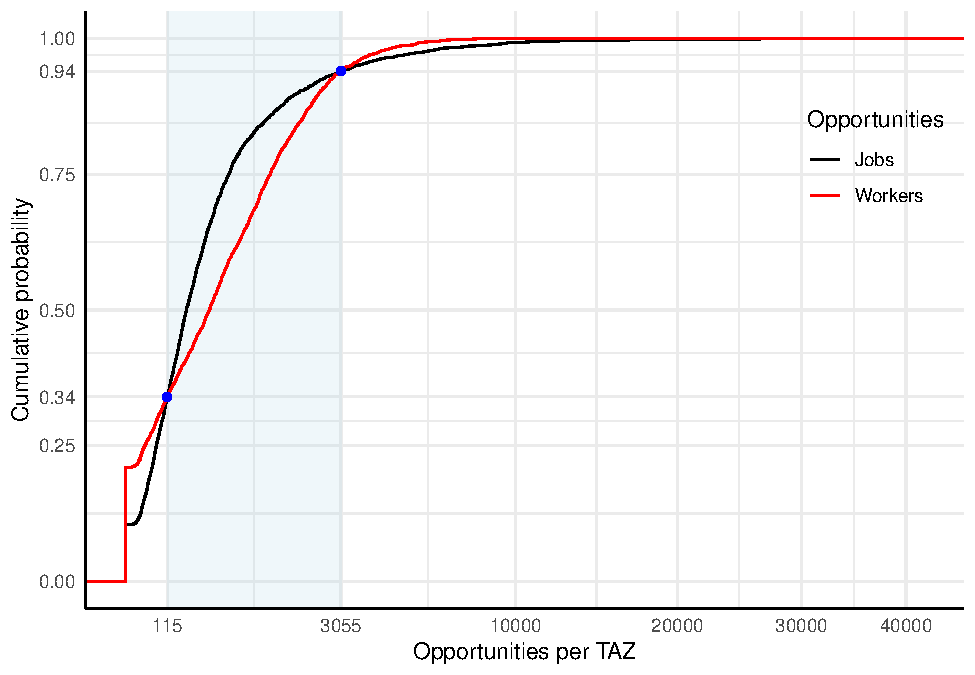
\includegraphics[width=1\linewidth]{Manuscript-Data-Package_files/figure-latex/ECD-plot-1} \caption{\label{fig:ECD-plot}The cumulative distribution of the number of jobs and workers per TAZ from the 2016 TTS data set. Light blue shaded ranges correspond to all cumulative proabilities where the number of workers per TAZ are larger than jobs per TAZ. }\label{fig:ECD-plot}
\end{figure}

Figure \ref{fig:tts-workers-jobs-plot} presents the number of workers
and jobs per TAZ. It can be observed that the spatial distribution of
jobs and workers is unequal, which is indicative of jobs-housing
imbalance, which can impact accessibility in a region
\citep{Levine1998rethinking}. Workers are concentrated in TAZ within the
center of the GGH and along the south-east and northern boarder of the
GGH. The center of the GGH corresponds to the Greater Toronto Area (GTA)
which is the most densely populated area in southern Ontario
\citep{statistics_canada_daily_2022}. The south east border of the GGH
neighbours Lake Ontario and is delineated by the urban built boundary of
the Ontario Growth Plan being home to the highest density of working
population in the GGH
\citep{ontario_built_2019, auditor_general_of_ontario_value_2021}. The
northern GGH border corresponds to the Simcoe, Dufferin, Kawartha Lake,
and Peterborough regions which are home to lower density of worker
population density population
\citep{auditor_general_of_ontario_value_2021}. Conversely, the spread of
jobs in the GGH is lower than the number of workers indicating
population is more spatially dispersed than jobs.

It can also be seen that from the bottom plot in Figure
\ref{fig:tts-workers-jobs-plot} that high to medium-low concentrations
of jobs are often present in the same areas as workers but only when the
scale is transformed. In other words, though there is a higher number of
TAZ with no workers than zones with no jobs (i.e., 791 TAZ with no
workers : 396 TAZ with no jobs) and the mean of workers per TAZ is
higher than the mean of jobs (i.e., 916 workers : 819 jobs) the number
TAZ with an extreme number of jobs at the highest and lowest percentiles
is significantly higher than the number of workers; see the following
cumulative probability distribution in Figure \ref{fig:ECD-plot} in
which the 94th to 100th percentile and the 0th to 34th percentile of
jobs in TAZ is higher than the number of workers in TAZ. This means that
between these ranges, TAZ have a higher number of workers than they do
jobs, echoing the more even spatial distribution of workers observed in
Figure \ref{fig:tts-workers-jobs-plot}.

\newpage

\hypertarget{calculated-travel-time}{%
\subsection{Calculated travel time}\label{calculated-travel-time}}

\{TTS2016R\} also includes travel time data for each home-to-work trip
as displayed in Figure \ref{fig:plot-tt-ttpertrip}. This travel time
corresponds to a car commute calculated using the R package \{r5r\} and
is interpreted as the travel time for a work commute for full-time
employed people in the GGH. The travel times were calculated assuming
the following input parameters: a maximum travel time less than or equal
to 180 mins (3 hrs) and a street network retrieved from OpenStreetMaps
for the GGH area. The 3 hr threshold was selected as it captures 99\% of
the trip taken (see the travel times summarized in Table
\ref{tab:TTS-16-desc-stats}).

It is important to note that all travel times within this data set are
calculated assuming car travel and one departure time for all origins.
These assumptions are not completely realistic since we know a small
proportion of trips are taken by non-car modes and travel time
departures varies, however, it is not possible from the data retrieval
system to obtain higher order tabulations that would allow us to split
the data further. Thus we do not know which trips are made with non-car
modes nor exact departure times in these tables. Though modal split and
travel times can be estimated through other methods
\citep[e.g.,][]{allen_suburbanization_2021, higgins2021changes}, for
simplicity, we assume that all trips are taken by one-time departure car
trip.

\begin{figure}
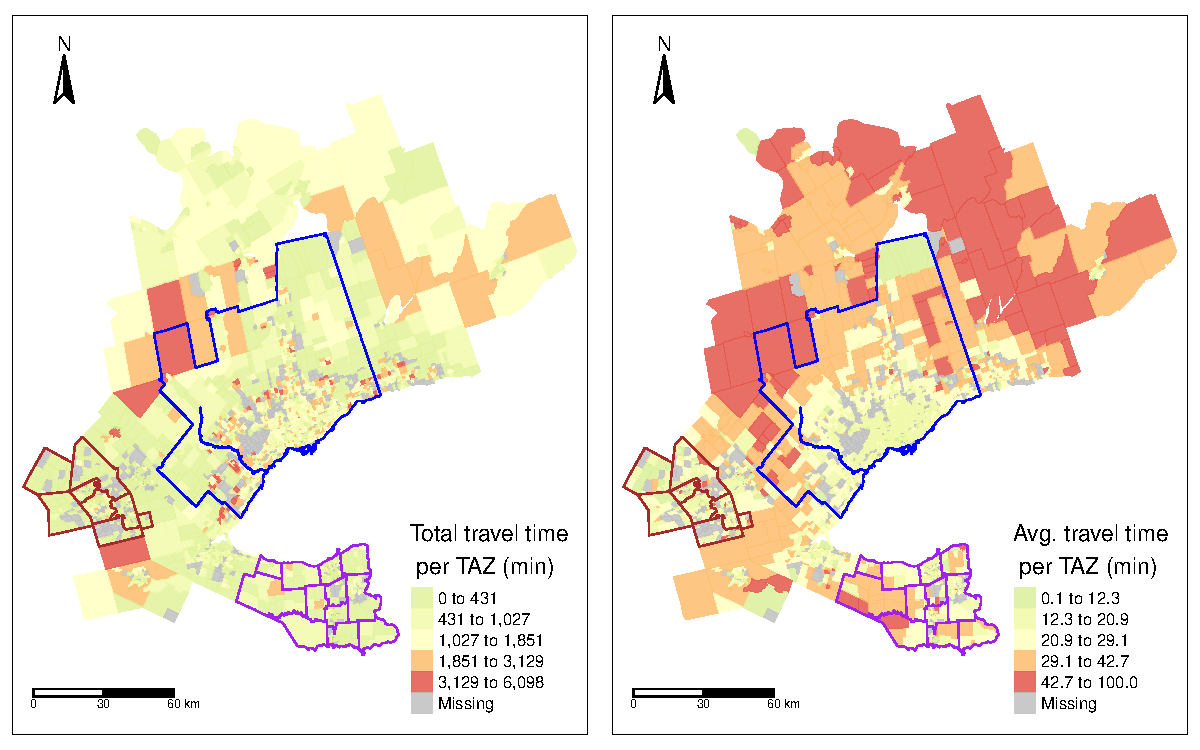
\includegraphics[width=1\linewidth]{Manuscript-Data-Package_files/figure-latex/plot-tt-ttpertrip-1} \caption{\label{fig:plot-tt-ttpertrip}Estimated total worker travel time (top) and average worker travel time (bottom) for each TAZ in the GGH.}\label{fig:plot-tt-ttpertrip}
\end{figure}

\newpage

As can be observed in Figure \ref{fig:plot-tt-ttpertrip}, the total
travel time (min) resembles the spatial trend distribution in the number
of employed people in the previous plot (Figure
\ref{fig:tts-workers-jobs-plot}). However, when the average travel time
per trip in each TAZ is presented, the spatial distribution is distinct
from all other plots presented so far. We can see that in areas around
the south-eastern border that make up the Greater Toronto and Hamilton
Area (GTHA) (e.g., Hamilton, Halton, Peel, Toronto, York, Durham) and
Niagara and Waterloo, the average travel times are moderately low.
Further from these areas, travel times are higher. Interestingly, even
in eastern areas (e.g., Peterborough) with high employment and high job
concentration, average travel time is higher than within the GTHA.

\hypertarget{calibrating-an-impedance-function}{%
\subsection{Calibrating an impedance
function}\label{calibrating-an-impedance-function}}

Impedance functions are useful to understand mobility behavior and are
part, for instance, of gravity models of spatial interaction
\citep{wilson1971, haynes_gravity_1985} and accessibility analysis in
many applications
\citep{hansen_how_1959, levinson_accessibility_1998, talen_assessing_1998, reggiani_accessibility_2011, paez_jobs_2013, kuai_examining_2017, barboza_balancing_2021}.
An origin destination matrix and a cost matrix (i.e., with travel times)
can be used in combination to estimate impedance functions. An impedance
function \(f(\cdot)\) depends on the cost of travel between locations
\(i\) and \(j\) \(c_{ij}\); it usually is a monotonically decreasing
function, although sometimes the function can increase to reflect
patterns of separation between activities; for instance, separation of
land uses means that very short commuting trips are relatively rare.
There can be sometimes also fluctuations due to hierarchical patterns,
where travelers bypass opportunities in favor of more distant
destinations that offer economies of agglomeration.

A useful technique to calibrate an impedance function is to use the trip
length distribution (TLD) as measured from origin-destination data
\citep{horbachov_theoretical_2018, batista_estimation_2019}. The TLD is
the representation of the likelihood that a proportion of trips are
taken at a specific travel cost. In our data set, where we assume cost
is travel time, the impedance function maps low travel times to higher
proportions of trips, and high travel times are mapped to low proportion
of trips.

In the GGH data presented, the empirical TLD (i.e., proportion of trips
taken vs.~travel time in minutes) is fitted to a density distribution
using maximum likelihood techniques and the Nelder-Mead method for
direct optimization available within the \texttt{fitdistrplus} package
\citep{fitdistrplus_2015}. Based on goodness-of-fit criteria and
diagnostics seen in Figure \ref{fig:TLD-Gamma-plot} and Figure
\ref{fig:plot-cullen-frey}, the gamma distribution is selected for the
presented data.

\begin{figure}
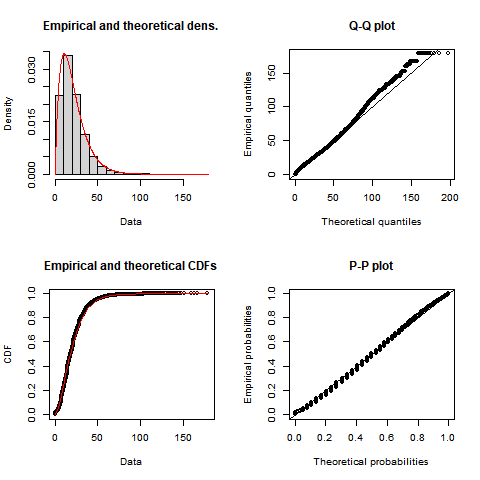
\includegraphics[width=1\linewidth]{images/impedance_function} \caption{\label{fig:TLD-Gamma-plot}Empirical TTS 2016 home-based car trip length distribution (black) and calibrated gamma distribution impedance function (red) with associated Q-Q and P-P plots}\label{fig:TLD-Gamma-plot}
\end{figure}

The resulting calibrated impedance function is given in the following
general form where the estimated `shape' is \(\alpha\) = 2.019, the
estimated `rate' is \(\beta\) = 0.094 , and \(\Gamma(\alpha)\) is
defined in Equation (\ref{gamma-dist}).

\begin{equation}
\label{gamma-dist}
\begin{array}{l}\ 
f(x, \alpha, \beta) = \frac {x^{\alpha-1}e^{-\frac{x}{\beta}}}{ \beta^{\alpha}\Gamma(\alpha)} \quad \text{for } 0 \leq x \leq \infty\\
\Gamma(\alpha) =  \int_{0}^{\infty} x^{\alpha-1}e^{-x} \,dx\\
\end{array}
\end{equation}

\begin{figure}
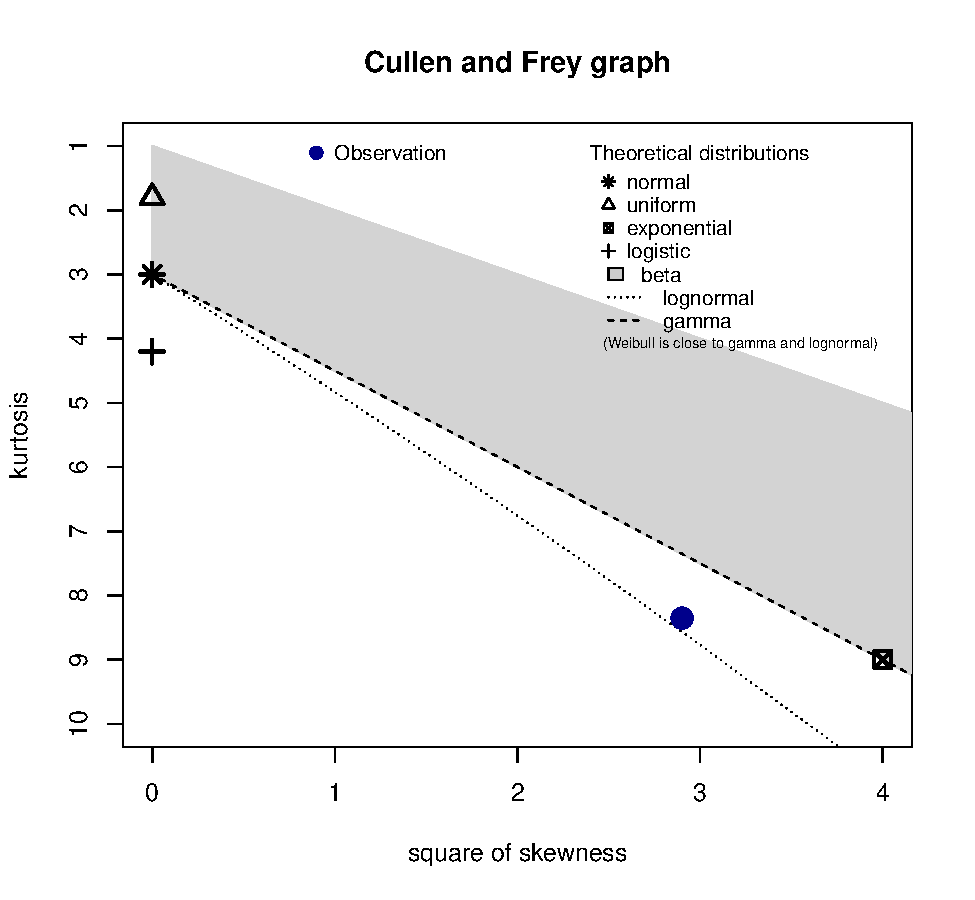
\includegraphics[width=1\linewidth]{Manuscript-Data-Package_files/figure-latex/plot-cullen-frey-1} \caption{\label{fig:plot-cullen-frey}Cullen and frey graphy for the 2016 TTS calculated travel times.}\label{fig:plot-cullen-frey}
\end{figure}

\begin{verbatim}
summary statistics
------
min:  0.1   max:  179 
median:  18 
mean:  21.4344 
estimated sd:  14.61254 
estimated skewness:  1.703326 
estimated kurtosis:  8.353363 
\end{verbatim}

\hypertarget{accessibility-to-employment}{%
\section{Accessibility to
employment}\label{accessibility-to-employment}}

As noted above, impedance functions are an essential component of
accessibility analysis. Equation (\ref{eq:conventional-accessibility})
shows that accessibility \(A_i\) is the weighted sum of opportunities
that can be reached from location \(i\), given the cost of travel
\(c_{ij}\). Summing the opportunities in the neighborhood of \(i\) as
defined by the impedance function \(f(\cdot)\), provides estimates of
the number of opportunities that can be reached from \(i\) at a certain
cost.

\begin{equation}
\label{eq:conventional-accessibility}
A_i = \sum_{j=1}^JO_jf(c_{ij})
\end{equation}

\noindent where:

\begin{itemize}
\tightlist
\item
  \(A\) is accessibility.
\item
  \(i\) is a set of origin locations.
\item
  \(j\) is a set of destination locations.
\item
  \(O_j\) is the number of opportunities at location \(j\). These are
  opportunities for activity and add some sort of \emph{supply} to the
  area;
\item
  \(c_{ij}\) is a measure of the cost of moving between \(i\) and \(j\)
\item
  \(f(\cdot)\) is an impedance function of \(c_{ij}\).
\end{itemize}

\begin{figure}
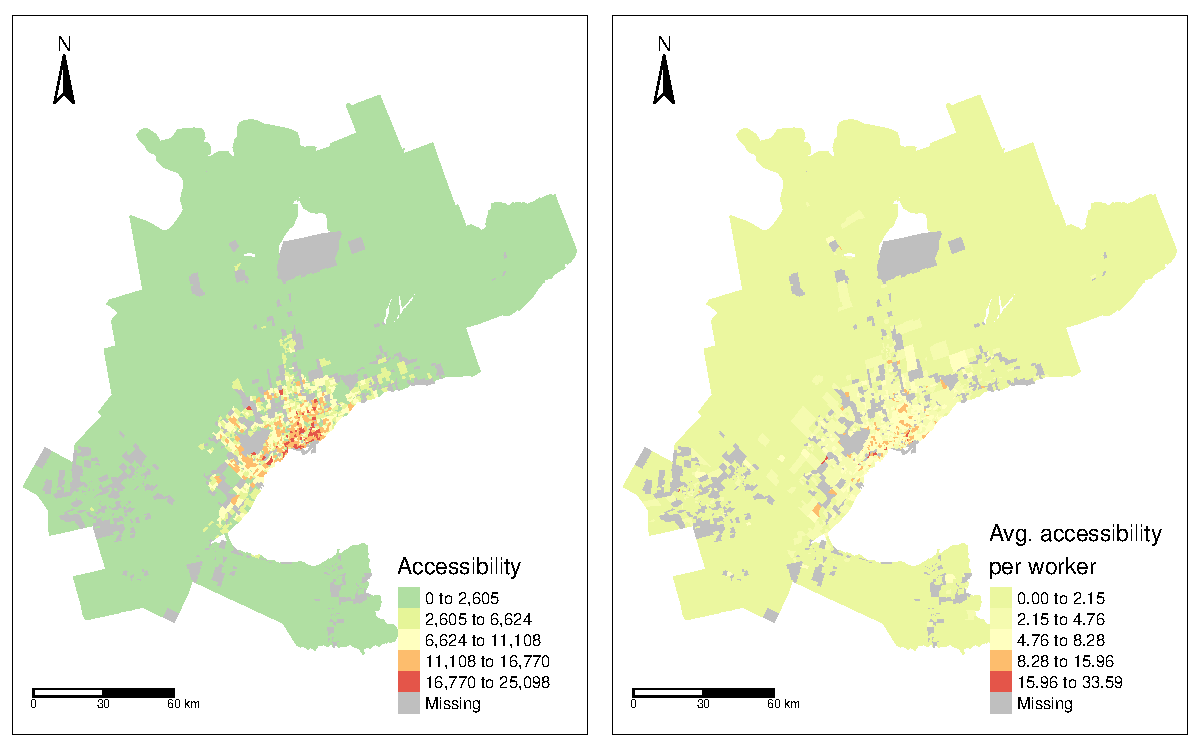
\includegraphics[width=1\linewidth]{Manuscript-Data-Package_files/figure-latex/plot-access-SA-GGH-TTS-1} \caption{\label{fig:plot-access-SA-GGH-TTS}Accessibility (top) and normalized accessibility (bottom) to employment in the GGH area}\label{fig:plot-access-SA-GGH-TTS}
\end{figure}
\newpage

Accessibility is a property of the origin (i.e., origin TAZ in our
data), the landscape of opportunities (i.e., the TAZ destinations in our
data), and transportation infrastructure (i.e., the travel time table).
Figure \ref{fig:plot-access-SA-GGH-TTS} presents the accessibility
estimates that result from the impedance function calibrated in the
preceding section. The top plot, that of the raw accessibility values,
presents a distinct radial trend where the majority of TAZ in and around
Toronto have high accessibility values and values gradually decrease in
TAZ which are further from Toronto's boundary. Alternatively, the bottom
plot in Figure \ref{fig:plot-access-SA-GGH-TTS} present the
worker-normalized accessibility values. In other words, the
accessibility value for each TAZ is divided by the number of workers in
each TAZ. The patterns in this plot are similar to the Greater Toronto
Area radial trend observed in the top plot but are less extreme (i.e.,
smaller spread).

\hypertarget{concluding-remarks}{%
\section{Concluding remarks}\label{concluding-remarks}}

The open data product introduced in this paper shares tables for
worker-to-employment data from the 2016 TTS aggregated by TAZ. In
addition, inter-centroid travel time tables are calculated, and the
planning/municipality boundaries are included to compliment the 2016 TTS
data. This open data product, \{TTS2016R\}, is freely available to
explore in an \texttt{R} environment. One possible use of these data, as
showcased in this paper, is the calibration of impedance functions which
in turn can be used for accessibility analysis.

New digital formats are increasingly complex and the explanation of the
methods often do not concisely and intelligibly fit within the confines
of a traditional article. With this motivation, we invite all who are
interested to use \{TTS2016R\} to explore the worker-employment patterns
contained in the \{TTS2016R\} package. In the spirit of novel and
original research, we hope readers value the efforts made to detail the
data in order to improve transparency in our work and encourage others
to replicate and, hopefully, inspire research of their own. We see this
product as providing open infrastructure for additional TTS or
complimentary data sets to be amended by the authors or wider
open-source community in the future.

\newpage

\bibliographystyle{sageh}
\bibliography{bibfile}


\end{document}
